\documentclass[10pt]{article}
\usepackage{icmlko}

\icmlmeta{IP 파운데이션 월드모델}{210}{지나간 세계의 숫자}{영화가 판에 들어오자 만화의 전이가 변했다 --- 0.2969는 유령도 오류도 아니라 시대 표기 없는 숫자였다}

\begin{document}

\twocolumn[
\icmlheader

\begin{abstract}
노트 852가 남긴 미결 하나: 833의 전이 앙상블 $0.2969$가 재현되지 않는다
(챔피언 경로는 $0.2561$). 유력 후보는 ``챔피언+TabPFN 앙상블''이라는
추측이었고, 867이 그것을 0순위로 올렸다. \textbf{그러나 833의 러너는
저장소에 보존돼 있었다} --- 열어 보니 TabPFN은 없고 챔피언 씨앗
4$\sim$7의 순위평균이었다(티처 \#34). 869가 망원 사슬로 격차를 갈랐다:
같은 재료에서 씨앗별 $\rho$ 12개가 852의 동결값과 자리수까지 일치하고
릿지 팔은 $0.3393$을 정확 재현하는데, 앙상블만 $0.2676$이 나왔다 ---
코드도 짝도 씨앗도 무죄. 창 안의 재료 변경은 정확히 하나, 837 재기선의
영화(KOBIS) 합류였다(티처 \#35). 870이 확정 시험을 돌렸다:
\textbf{영화 한 도메인을 빼고 재구성하자 $0.2969$가 소수 넷째 자리까지
돌아왔다($|\Delta|=0.0000$).} 숫자는 유령이 아니라 \emph{지나간 세계의
숫자}였다. 처방은 둘이다 --- 적합을 낳는 러너는 짝 라벨 지문만이 아니라
\textbf{학습측 재료 지문}을 남긴다(era manifest 동결), 그리고 아카이브의
숫자를 인용할 때는 시대를 함께 적는다.
\end{abstract}
]

\section{세 사이클의 해부}

\textbf{869(분해).} 격차 $0.0408 = E_1 - 0.2561$을 망원 사슬
$(E_1{-}E_2)+(E_2{-}E_4)+(E_4{-}E_5)+(E_5{-}0.2561)$로 갈랐다 ---
잔차는 구조상 0이다. 실측: 씨앗 부분집합 $+0.0120$ · 순위결합
$-0.0005$ · 앙상블화 $-0.0003$ · 재료 $+0.0004$. 그러나 재현 갈래가
먼저 실패했다($E_1=0.2676 \neq 0.2969$) --- 사전등록대로 주범 선언을
멈추고 구현을 의심했다.

\textbf{해부(무죄 4면).} 순위평균 코드는 git에서 불변, 스크래치의
ff753은 보존본과 diff 0, 씨앗별 $\rho$ 12개는 852와 자리수까지 일치,
그리고 릿지 팔은 $\alpha$까지 포함해 $0.3393$을 정확 재현 --- 짝 쪽
데이터가 833 시대와 동일함을 증명한다. 남는 설명은 하나: 판의 학습
재료가 움직였다.

\textbf{물증(티처 \#35).} 833 측정(8/7 21:55)과 852(8/8 11:31) 사이
창에서 재료를 바꾼 커밋은 정확히 하나 --- kobis\_axes.json 26{,}612행
(8/7 23:39)과 837의 tri\_domain 영화 절이다. 기제 사슬:
$\mathrm{base()} \to \mathrm{\_idol} \to \mathrm{harness.load} \to
\mathrm{tri\_domain.load\_all}$ --- 합동 적합에 12번째 도메인이 들어오면
만화 짝의 예측이 변한다.

\textbf{870(확정).} 런타임 패치로 영화만 빼고 833 세계를 재구성해
같은 4씨앗을 다시 적합했다. $E_1^{\mathrm{recon}} = 0.2969$,
$|\Delta| = 0.0000$.

\begin{figure}[t]
\centering
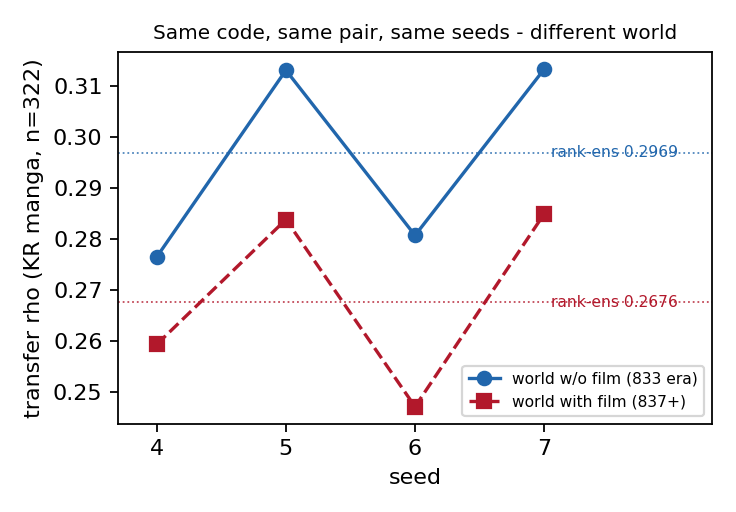
\includegraphics[width=\linewidth]{figs/pastworld.png}
\caption{같은 코드·같은 짝·같은 씨앗, 다른 세계. 영화 합류 전(파랑)
씨앗별 전이 $\rho$는 4/4 모두 합류 후(빨강)보다 높고, 순위평균
앙상블은 $0.2969 \to 0.2676$으로 움직인다. 병기 관측: 영화 합류가
KR 만화 A-경로 전이를 $\sim$0.03 낮췄다(SE 없음 --- 주장 아님).}
\end{figure}

\section{교훈}

\textbf{시대 표기 없는 숫자가 유령을 만든다.} 852는 ``스크래치 소실로
원인 확정 불능''이라 적고 TabPFN 추측을 남겼다. 그 추측이 두 사이클
뒤 0순위 좌표에 박혔고, 하마터면 러너·산출물·등록이 3점 보존된 숫자를
``유령''으로 강등할 뻔했다(티처 \#34가 적발). 재료가 자라는 실험실에서
숫자는 세계에 상대적이다 --- \textbf{era manifest}(도메인별 학습
행수·라벨 해시)를 동결해 두면 다음 시대 단절은 5분 진단이 된다.

\textbf{갈래가 판정을 지켰다.} 869의 사전등록은 재현 실패 시 주범
선언을 금지했다 --- 그 금지 덕에 ``씨앗이 주범''이라는 그럴듯한 반쪽
결론 대신 시대라는 진짜 원인에 도달했다. 866의 도달 불능 갈래,
868의 문면 구멍에 이어, 갈래 3속성(배타·도달·전역)이 실전에서 값을
지불한 세 번째 사례다.

\textbf{서빙 함의는 없다.} 정본 전이 상수는 B-경로 무정체
$0.3919$(852)로 불변이다. 이 아크가 바꾼 것은 숫자가 아니라
숫자를 읽는 법이다.

\end{document}
